A major goal of this model is to study the effect that leakage has on optimal
tunnel configuration. The Hyperloop infrastructure will be designed and
manufactured with the goal of making the tube air tight; however, a perfectly
air tight tube is likely not possible. Slight leakage flow rates are to be
expected due to diffusion, desorption, permeation, leaks through micro cracks,
and leaks in mechanical mechanisms. Furthermore, air will likely need to be
introduced to the system to allow passengers to board. The leakage rate due to
diffusion and permeation is proportional to the tube surface area while the air
introduced into the system during passenger boarding is proportional to the
size of the boarding area and the frequency at which pods are boarded by passengers.
Thus, it is reasonable to assume that leakage rate is proportional to pod size
and the frequency at which pods leave the station. While the exact leakage rate
into the system is difficult to quantify, accounting for leakage provides
valuable insight to performance of the system as a whole.
The previous trade study showed that, for a given leakage rate, an operating
pressure exists at which steady state energy consumption is minimal.
This is because an increase in pressure decreases the energy required by the
vacuum pumps to maintain tube pressure while increasing the energy required by
the compressor system onboard the pod to compress higher mass flows.
The pressure at which this minimum occurs is a function of leakage rate.
To evaluate the sensitivity of optimum pressure to leakage rate, the previous
study will be repeated for a range of leakage rates. In each study, the
pressure at which minimum energy consumption occurs will be determined using
the ScipyOptimizer. The minimum value of total energy cost and the
corresponding tube pressure will be recorded and plotted to evaluate the
effects that leakage rate has on the system design variables.

% \begin{figure}
% 	\centering
% 	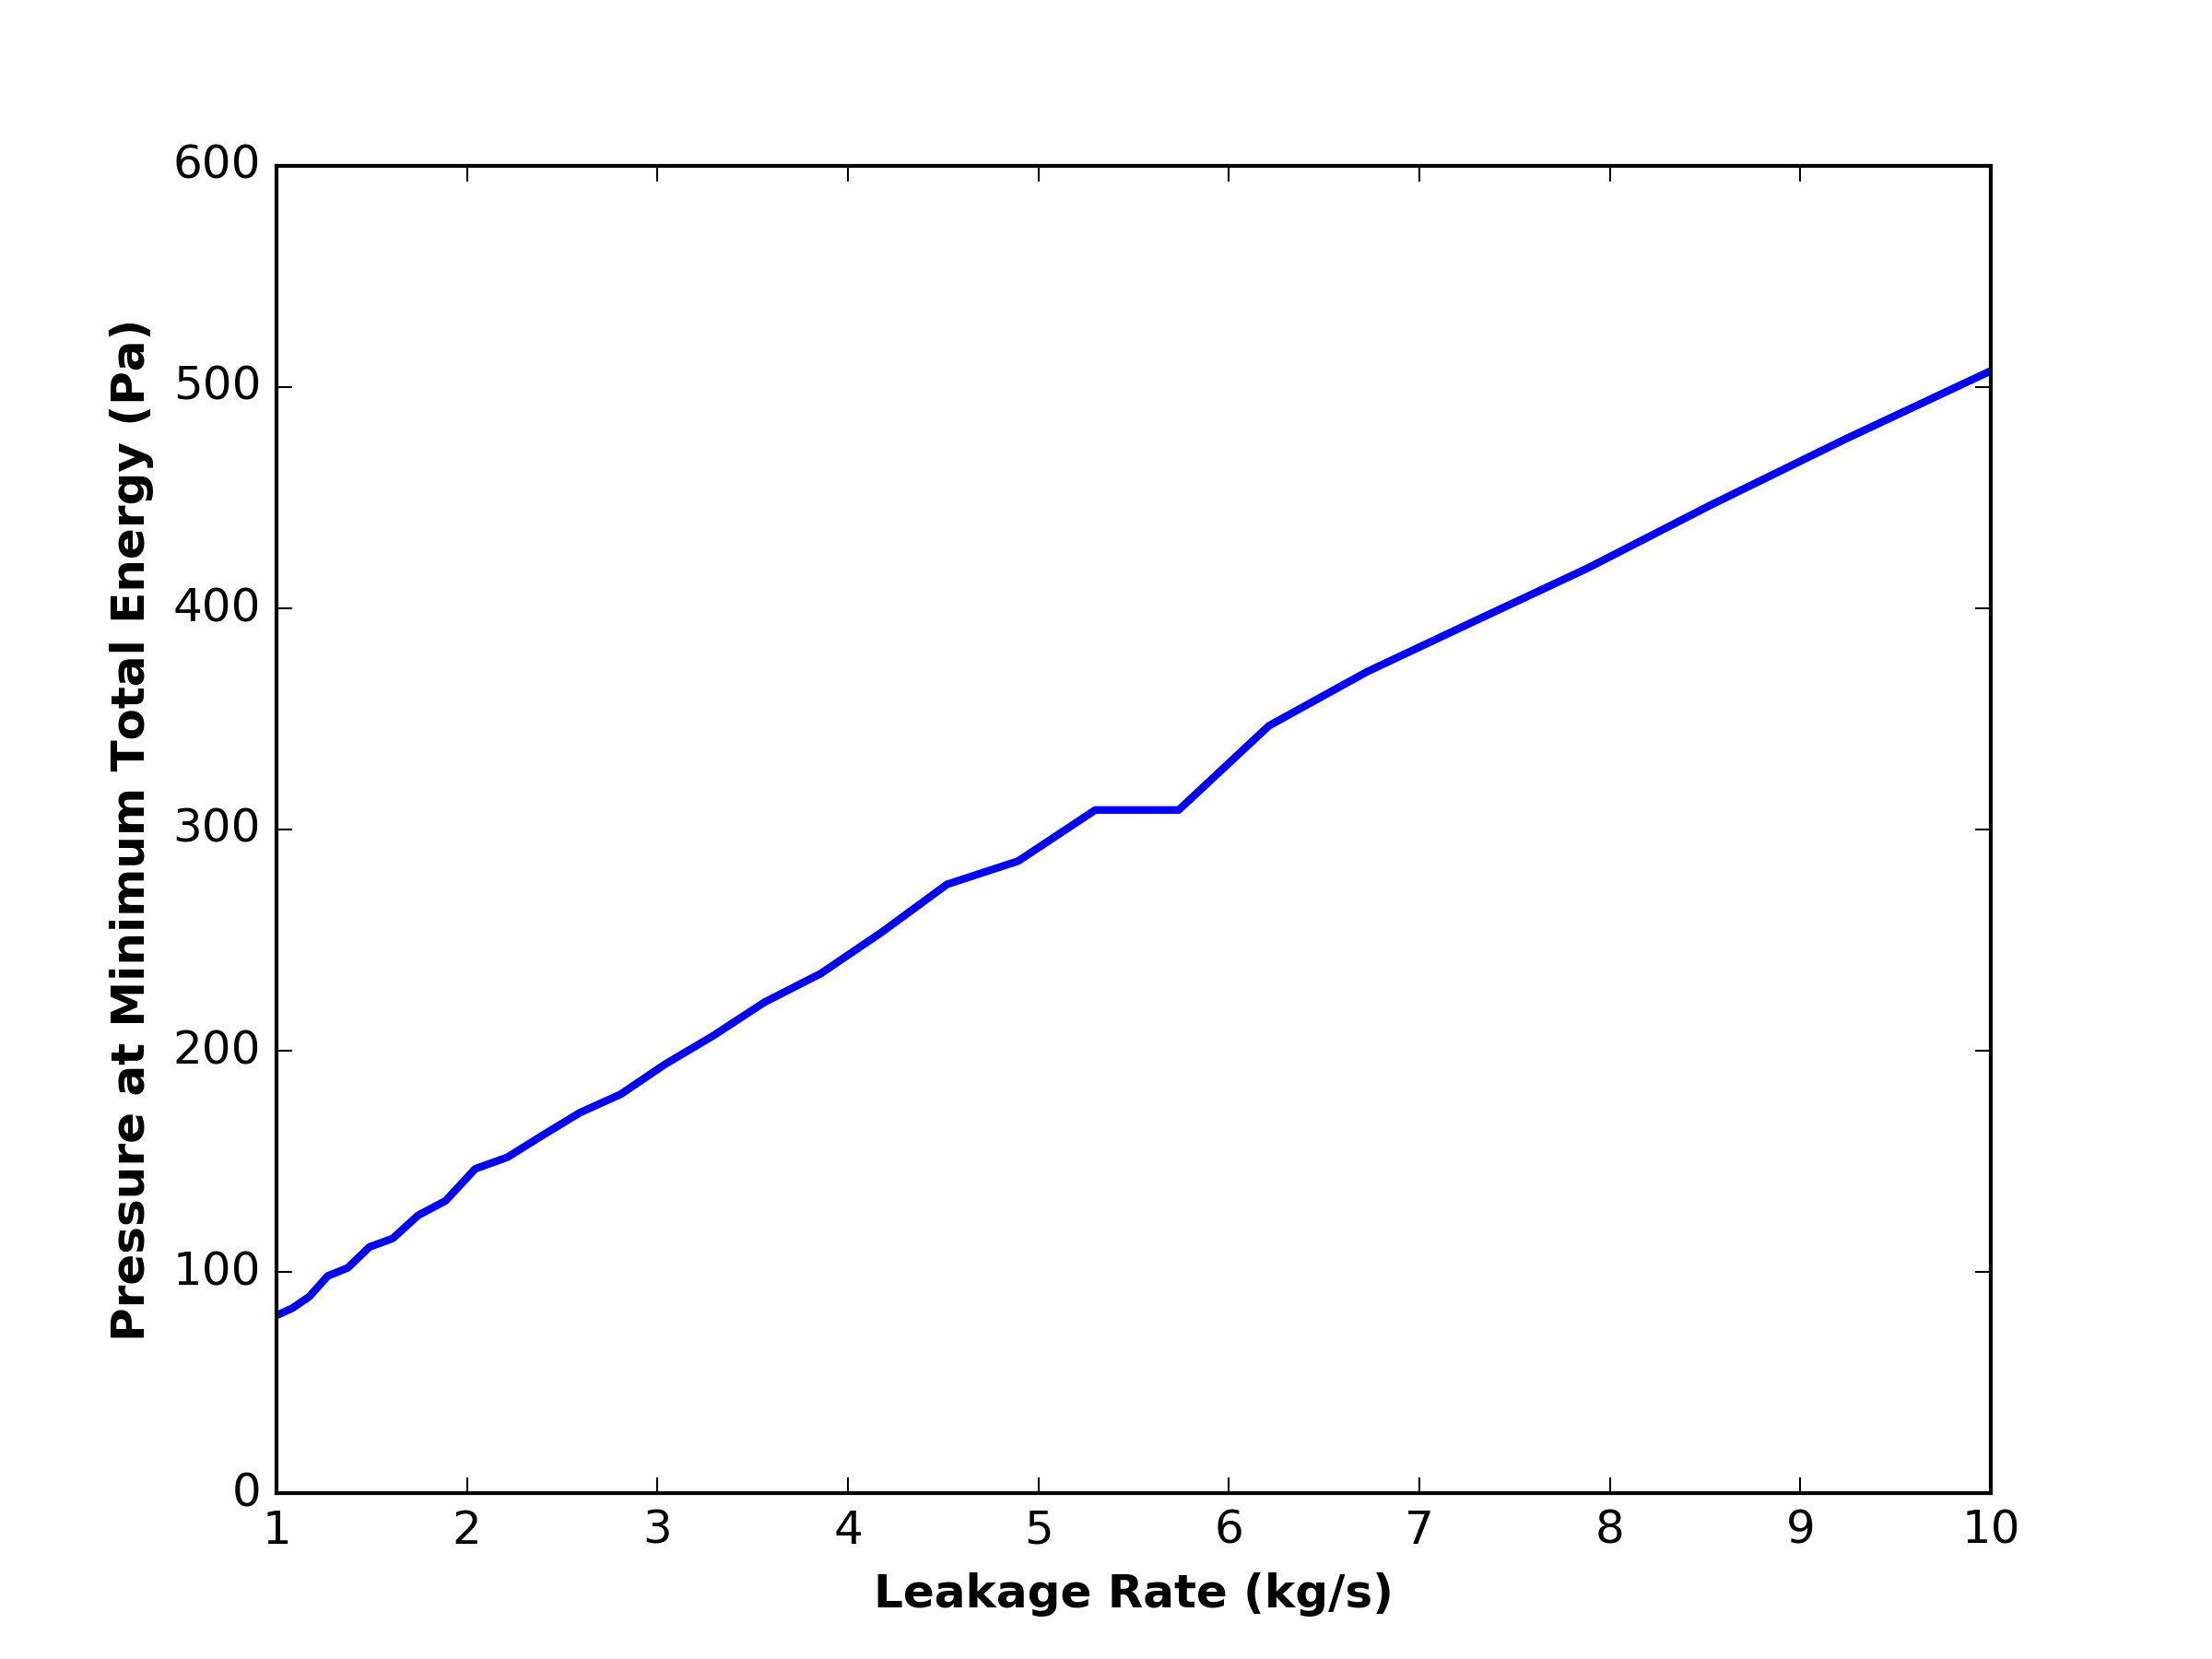
\includegraphics{../../images/graphs/leakage_trades/leakage_vs_pressure.png}
% 	\caption{Pressure at Minimum Energy Consumption vs. Leakage Rate}
% 	\label{fig:pres_vs_leakage_rate}
% \end{figure}
\begin{figure}
	\centering
	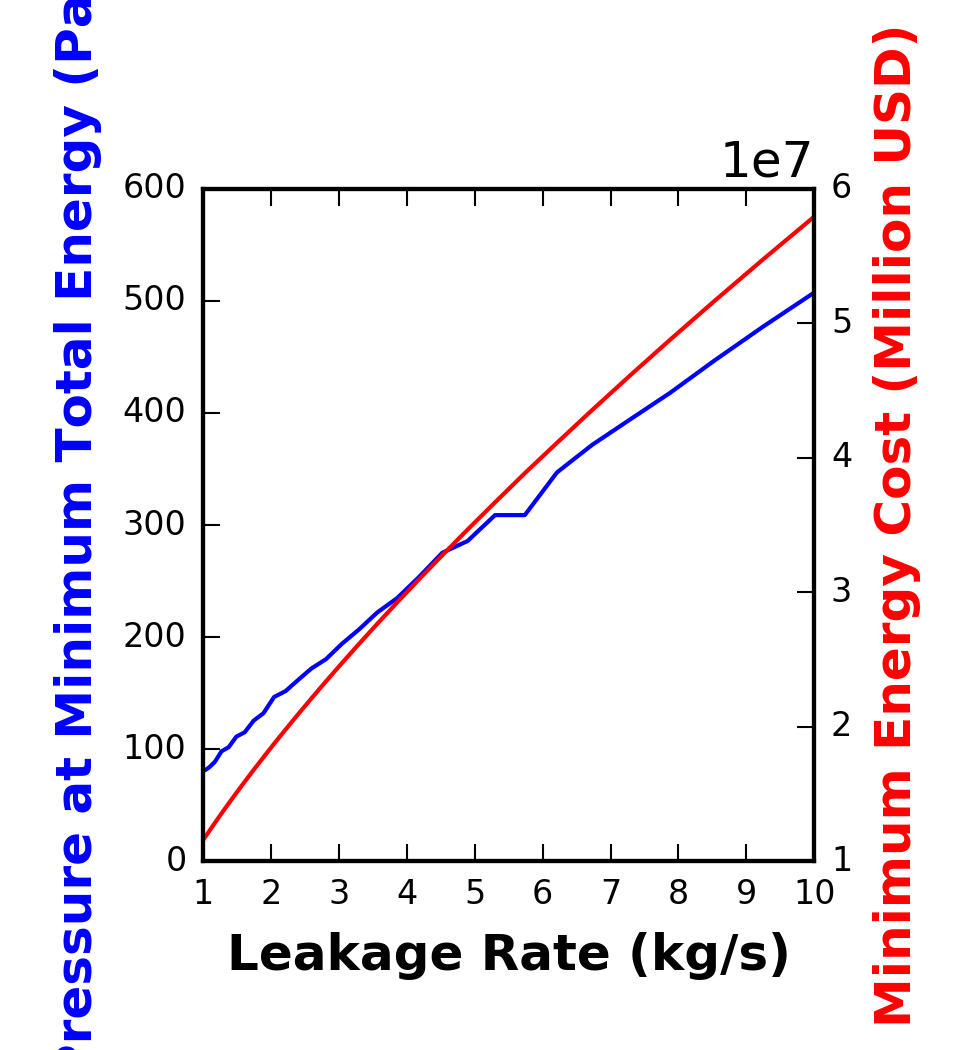
\includegraphics{../../images/graphs/leakage_trades/leakage_rate.png}
	\caption{Minimum Energy Cost vs. Leakage Rate}
	\label{fig:pres_vs_leakage_rate}
\end{figure}
\Cref{fig:pres_vs_leakage_rate} shows the pressure at minimum energy
consumption vs. the leakage rate of the tube. The tube pressure that optimizes
cost increases as leakage rate increase. This trend is reasonable because
increasing leakage rate increases the power required for the vacuum pumps to
maintain the tube pressure, which is offset by increasing the pressure that the
vacuum is required to maintain. This relationship is critical because it
reveals a coupling between tunnel leakage and energy consumption that system
designers must consider. As \cref{fig:pres_vs_leakage_rate} reveals, changes
in leakage rate can have a significant effect on energy consumption and energy cost.
Increasing leakage rate causes minimum energy consumption to increase
significantly, with the cost increase being even more substantial when
operating at a suboptimal pressure. If the designer wants to optimize the
system by minimizing the energy consumption, then more accurate modeling or
empirical studies will be necessary to determine operating pressure.
Furthermore, the assumption made in this study that leakage rate is constant is
likely not indicative of a real system. As pod frequency changes, the
leakage rate, and therefore the optimal pressure of the tunnel, is also likely to change.
It may be possible for system designers to account for variable tube pressure
when sizing the battery, compressor motor, and tube diameter in order to give
the operator flexibility to change the tube pressure with pod frequency.
This would allow the Hyperloop system to adapt to changing operating conditions
to more closely track optimal design configurations in real time.
Further research with higher fidelity modeling is necessary to further
characterize the benefits of variable tunnel pressure as it relates to pod frequency and leakage.
